%%%%%%%%%%%%%%%%%%%%%%%%%%%%%%%		CHAP 2		%%%%%%%%%%%%%%%%%%%%%%%%%%%%%%%

\chapter{The ANNIE Experiment}
\label{cha:2}
\textcolor{blue}{have to clean this too.}

The \textbf{A}ccelerator \textbf{N}eutrino \textbf{N}eutron \textbf{I}nteraction %
\textbf{E}xperiment (ANNIE) will provide a complementary measurement of final-state %
neutron abundance from pure neutrino interactions and neutron yields in relation to %
the energy and direction of final-state muons with respect to the original neutrino.
ANNIE can accomplish this task, currently poorly-known and difficult to measure.
These combined data can be used to better constrain nuclear models of neutrino interaction %
physics and are an essential input to Monte Carlo models, used for calculating %
detection efficiencies, expected background rates, accurate limits, and confidence levels.
The count of neutrons can also be used to reject contamination by atmospheric %
neutrino interactions in proton decay experiments and in a sample of diffuse supernova %
background neutrinos and may also help to statistically address wrong-sign contamination %
in oscillation analyses.
In addition to helping understand fundamental neutrino-interaction physics, tagging events %
by the presence and number of final-state neutrons can provide physics analyses with a better %
handle for signal-background separation and even allow for discrimination between %
different types of neutrino interactions.

The ANNIE experiment consists of a small water Cherenkov detector, instrumented
with both conventional photomultiplier tubes (PMTs) and eventually LAPPDs.
A downstream Muon Range Detector (MRD) is also installed in the hall.
Neutron tagging in Gadolinium-doped water may play a significant role
in reducing backgrounds from atmospheric neutrinos in next generation 
proton-decay searches using megaton-scale Water Cherenkov detectors.
Similar techniques might also be useful in the detection of supernova neutrinos. 
Accurate determination of neutron tagging efficiencies will require a 
detailed understanding of the number of neutrons produced by neutrino interactions 
in water as a function of momentum transferred.
ANNIE is mainly designed to measure the neutron yield of atmospheric neutrino interactions 
in gadolinium-doped water.
An innovative aspect of the ANNIE design is the use of precision timing to 
localize interaction vertices in the small fiducial volume of the detector.
We propose to achieve this by using early production of LAPPDs 
(Large Area Picosecond Photodetectors).
This experiment will be a first application of these devices demonstrating
their feasibility for Water Cherenkov neutrino detectors.

The ANNIE experiment is a prototype neutrino detector %
currently taking data Fermilab USA.
It aims to be a test bed %
for many new technologies from Gd-doped water %
interaction of neutrons to the use of early prototype %
LAPPDs (Large Area Picosecond Photodetectors) %

The ANNIE experiment consists of a small, economical Water Cherenkov detector, instrumented %
with both conventional photomultiplier tubes (PMTs) and LAPPDs, and deployed on the intense %
Booster Neutrino Beam (BNB) at Fermilab.
The experiment is planned to proceed in two stages: 
\begin{itemize}
  \item[\bfseries Phase I] a partially-instrumented test-beam run using only PMTs %
    for the purpose of measuring critical neutron backgrounds to the experiment;
  \item[\bfseries Phase II] a longer run with a more fully-instrumented detector %
    where incremental research and development for the LAPPDs and %
    accompanying fast electronics will be fulfilled, as long as the expansion of the %
    photodetector coverage (both LAPPDs and PMTs) required.
\end{itemize}

Year 1 will focus on the R\&D, particularly tests of the first available LAPPDs in water.
Installation of the first LAPPDs and a significant fraction of the additional PMTs, as %
well as the calibration system, will take place in Year 2.
Data-taking would commence in Year 3 and continue through Year 5, with the physics reach of %
the detector increasing as the fraction of LAPPDs increases over time.
Publication of derived results would occur by the end of Year 5.


\section{Water tank}
\label{2.2}
\textcolor{red}{tank = PMTs, water, future LAPPDs and Gd (NCV). Very messy now}

The main component of the experiment is the water tank, installed in the SciBooNE hall %
at Fermilab.
Incom Inc, the company selected to commercialize the LAPPD photodetectors, has provided a
quote to the ANNIE collaboration committing to produce 20 detectors
This is already price-competitive per unit area with equivalent
technologies offering similar capabilities (a single LAPPD covers 16 times the area of a 10k 2”
Photonis Planacon MCP-PMT and 64 times that of an 8k Hamamatsu 1 inch tube).
These early LAPPDs will be produced in small batches over a period of several years, %
with the first two LAPPDs arriving no later than September 2016 and 5-8 more tiles in September 2017.
Specifications of the LAPPDs are derived from prior tests: time resolutions below 100 psec, %
spatial resolutions below 1~cm, and gains above 1x10 7 [21], as well as 20\% quantum %
efficiency photocathodes and good gain uniformity [32].
The LAPPD purchase by the ANNIE collaboration represents a technology investment that will %
pay out past its experimental lifecycle.
Their use in ANNIE provides an essential proof-of-principle %
demonstration of the technology and LAPPDs purchased through ISU can be made available for %
future HEP efforts after ANNIE.
Application-specific detector development work necessary to deploy LAPPDs for use %
in water is also required.
The devices need to be characterized and—along with their high voltage connections %
and front-end readout boards—must be mounted and placed in the water volume.%
Water submersion tests (including tests using the full ANNIE water volume) will proceed %
first using several 6~cm photosensors provided by ANL, built using a similar design and %
process to the Incom LAPPDs.
14ANL will also design and provide an 8” x 8” structure on which to mount the 6~cm tiles, %
compatible with the waterproof housing for full-size detectors.
The additional development of electronics to read out the LAPPDs and its impact on the %
overall DAQ system is described in Sec 4.7.
One or more publications on the novel instrumentation of ANNIE are planned.
In order to guarantee physics results from this effort independently of the status of LAPPD %
production, an alternative choice for light detectors will be developed in parallel.
The optimal choice at this stage would appear to be the Hamamatsu H11934-200 ultra %
bialkali 1-inch PMTs.
With a quantum efficiency of 43\%, comparable photon collection efficiencies to %
LAPPDs can be achieved with less spatial coverage.
The combination of 270 psec time resolutions and fine granularity of these detectors %
provides capabilities comparable to those discussed in Sec 3.4 (see Fig 6).
A quote for 600 of these tubes has been obtained from Hamamatsu and is comparable in cost %
with the equivalent area x coverage scenario proposed with LAPPDs.
It would rely on the same electronics, and mixed 1-inch and LAPPD scenarios are also possible.
The group at Lawrence Berkeley National Laboratory (LBNL), led by PI Orebi Gann, %
is already working with these tubes in a bench-top scale water-based liquid %
scintillator setup aimed at demonstrating ring imaging for high-energy events in this target medium, %
leveraging funding by the LBNL LDRD program.

Photodetection in ANNIE Run I will be provided by of 60 8 Hamamatsu PMTs, from a stock of %
Super-K spares

\textcolor{red}{Improve Gd section.}
Gadolinium in water (NCV)
EDGAS and other experiments.
The Super-Kamiokande (SK) [1] is the largest light water Cherenkov detector %
that has been successfully observing solar, atmospheric and accelerator neutrinos.
Recently the addition of 0.2\% of a water soluble gadolinium (Gd) compound to SK %
has been proposed [2].
This modification can greatly improve the detection sensitivity of anti-electron neutrinos.
The inverse beta interaction in the water, emits a positron and a neutron.
The positron, radiating Cherenkov photons, is immediately detected.
The neutron is quickly thermalized in the water, and is then captured by Gd with a %
probability of 90\%.
Upon capturing a neutron the Gd emits 3-4 gamma rays having a total energy of %
about 8 MeV.
The time and spatial correlation of the positron and neutron capture events (20 us and 4 cm) %
can significantly reduce the backgrounds, and hence enhance the nu e signal events.

\subsection{Photodetectors+LAPPDs}
\label{2.2.1}
Photomultiplier tubes
As noted earlier, ANNIE Phase II will achieve the necessary coverage to detected neutron capture
in Gd-loaded water using by: (1) utilizing twenty in-hand 11-inch L PMTs (refurbished %
proto-types developed under R\&D grants from the NSF and DNN), (2) purchasing 50 new HQE 10-inch %
Hamamatsu PMTs (45+5 spares), and (3) re-using the 8-inch Hamamatsu PMTs refurbished by %
UC Irvine for ANNIE Phase I.
We request funds to purchase the HQE 10-inch PMTs, but with a reserve option to purchase %
140 new 8-inch normal QE PMTs (the higher-cost, higher-channel-density option).
More detailed simulations will enable a final decision by the collaboration before %
procurement of the conventional PMT system.
Calibration, testing and installation of these PMTs will be carried out by UC Davies and/or UC Irvine.

List of pmts employed??

Talk about LAPPDs

\section[MRD and VETO]{Muon Range Detector+Veto}
\label{2.3}
\textcolor{red}{mostly ok, I guess I have every information.}

A Forward Anti-Coincidence Counter (FACC) consisting of two layers of overlapping muon %
paddles detects charged particles produced in the dirt upstream of the hall.
This allows the rejection of events in the tank unrelated to the beam.

An iron-scintillator sandwich muon range detector (MRD), already in the experimental hall, %
will be used to range out and fit the direction of daughter muons from neutrino interactions %
in the water target.
Neutrino interactions in the water target will produce light with no signal in the FACC and those
that are muon neutrino charged current will likely produce a muon going through the MRD.

The role of the Muon Range Detector is to confine the muons produced in charge-current %
quasi-elastic (CCQE) interactions, which is the dominant process in SciBooNE.
By confining the muon its energy can be reconstructed thus giving a handle on the neutrino %
energy.
The MRD consists of 13 alternating horizontal and vertical scintillator planes, %
each separated by a 5~cm iron sheet.
This results in 60~cm of absorber equivalent to %
stopping a 1 GeV muon.
The first plane is directly downstream of the EC allowing for %
better track matching and energy reconstruction of pai0 decay photons that escape the EC. 
Three planes are required to be hit for a track to be reconstructed in the MRD, equivalent %
to approximately a 180~MeV muon.
The total mass of the detector is 60 tonnes, of which %
approximately 48 tonnes is absorber.
Planes can be moved forward or backward via the use %
of winches attached to the side of the support frame.
There are 362 channels in total; 182 horizontal, 180 vertical.
Each channel is 20 cm wide and either 155 cm (horizontal) or 138 cm (vertical) long.
Planes have active areas of 310per260 cm 2 (horizontal) and 300per276 cm 2 (vertical).
Of these 362 channels 5 different photomultiplier tubes (PMTs) are used.
The horizontal planes consist of 14 stage EMI 9954KB PMTs from the KTeV experiment, %
as well as EMI 9839b and 9939b PMTs.
The vertical planes consist of 10 stage Hamamatsu 2154-05 PMTs from %
the NuTeV experiment and RCA 6392A PMTs.
The electronics consist of LeCroy 4300B ADCs, LeCroy 3377 %
TDCs and the LeCroy 1440 high voltage system.

ANNIE makes use of an existing Muon Range Detector (MRD) that remains mostly intact in the %
experimental hall.
The MRD is a steel and plastic scintillator sandwich detector, designed to range %
GeV-scale muons and provide directional information.
The electronics and high voltage %
(both for the MRD and photosensors in the water volume) will be provided by Fermilab PREP %
for the duration of the experiment.
Several layers of muon paddles and PMTs are absent; Fermilab has agreed to provide %
materials and instructional support to the ANNIE collaboration to replace the %
missing paddles.

\begin{wrapfigure}{L}{0.5\textwidth}
  \centering
  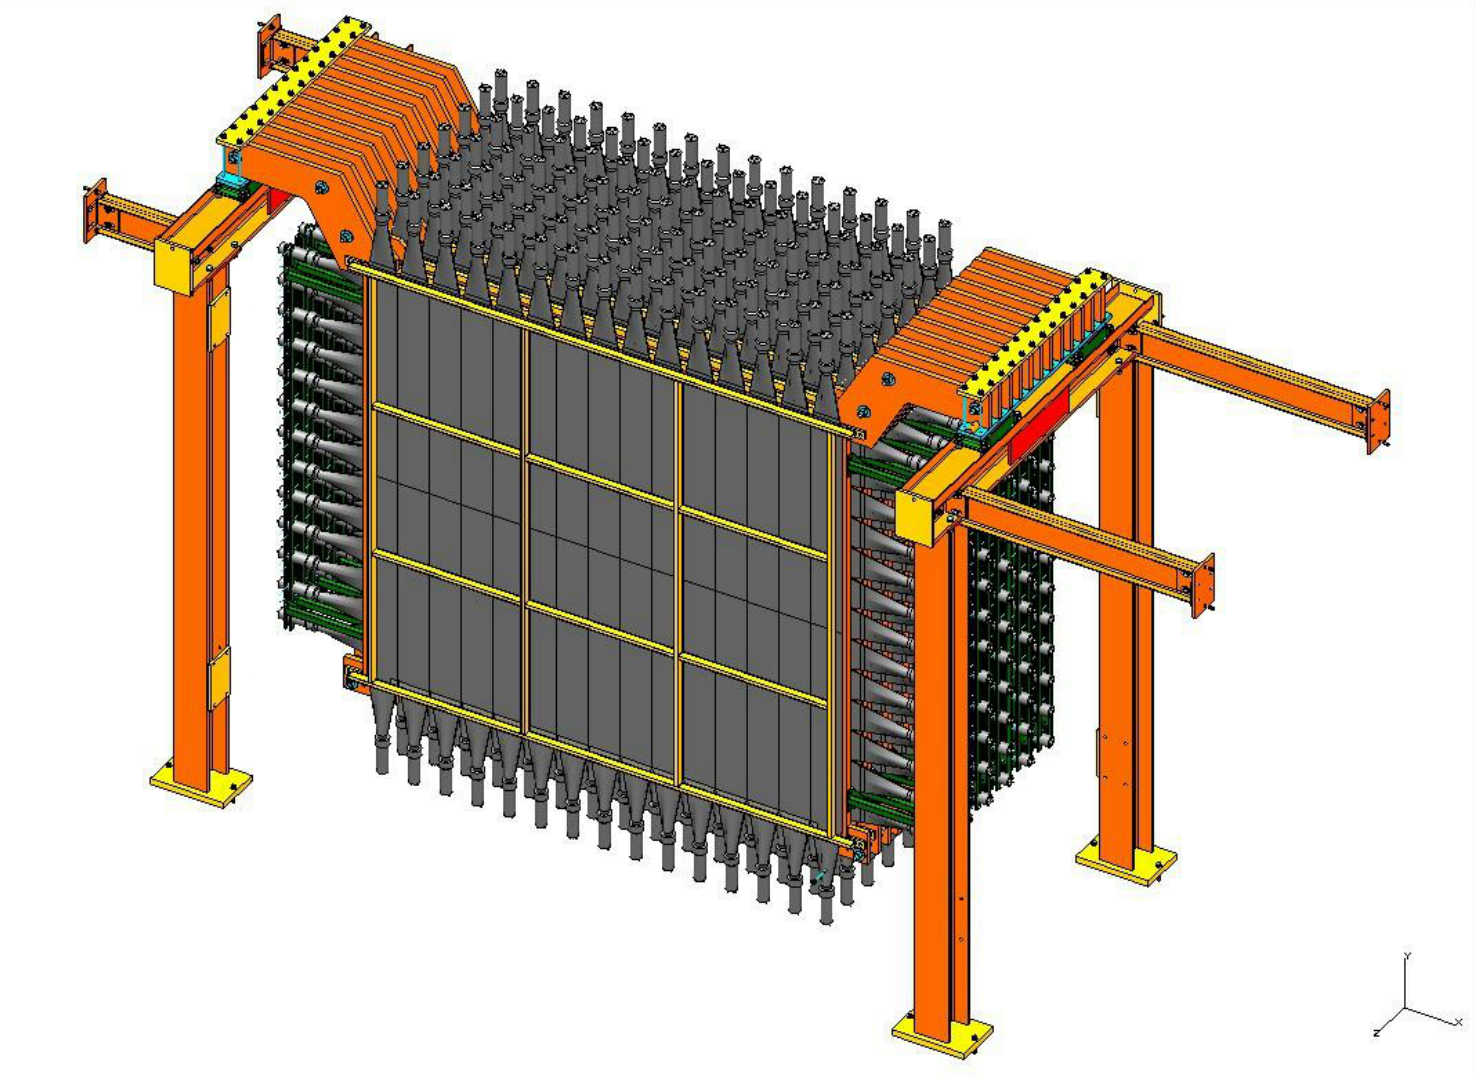
\includegraphics[scale=.15]{pics/pag23Nakajimathesis}
  \caption{Drawing of the MRD.}
  \label{fig:mrd}
\end{wrapfigure}


A fraction of the MRD will be made operational for Phase I of ANNIE in early fall.
Refurbishment activities by UC Davies will be scheduled after this phase is completed taking %
so that the detector system is fully operational in time for ANNIE first physics runs.
ANNIE will rely on a Forward Anti-Coincidence Counter (FACC) consisting of 2 layers %
of overlapping muon paddles to reject charged particles produced in dirt, upstream of the hall.
Fermilab provided a stock of 60 muon paddles taken from the CDF experiment, from which a subset %
of 26 paddles were systematically tested and selected.
These paddles have already been attached to the wall by students from UC Davis with %
the help of Fermilab technicians, using standard 80/20 aluminum extrusions and brackets, %
arranged in two staggered layers of 13 paddles each.

\begin{figure}[]
  \centering
  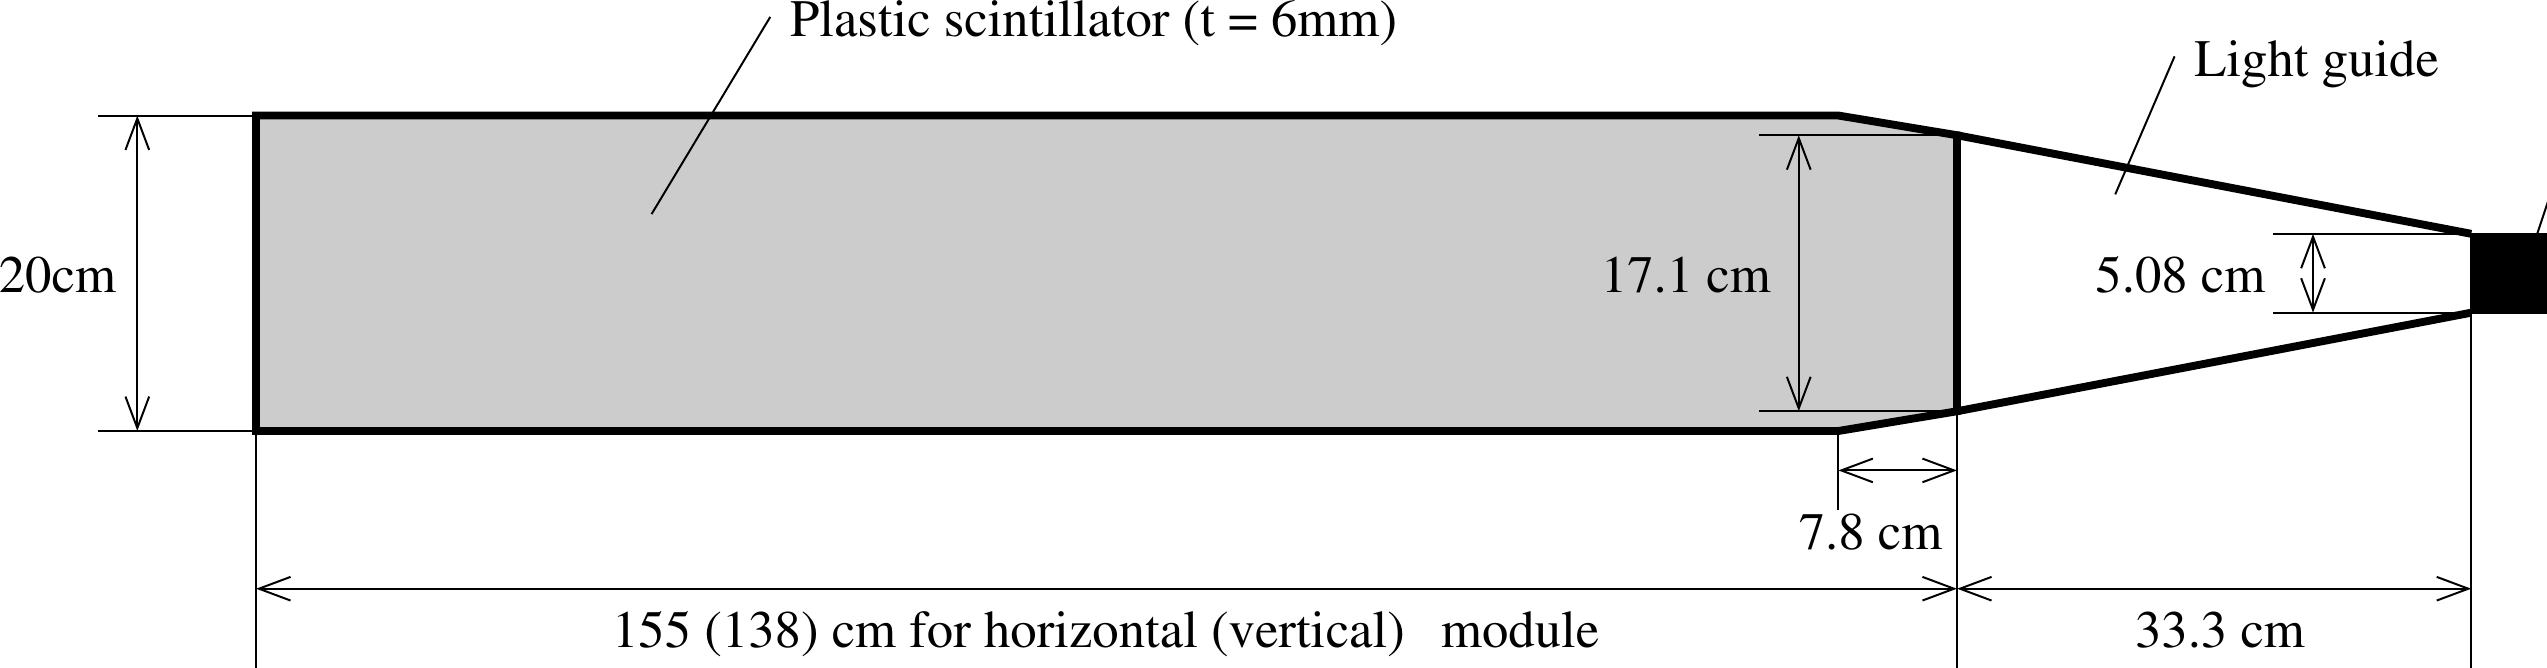
\includegraphics[scale=0.20]{pics/pag24Nakajimathesis}
  \caption{Paddle used for the MRD.}
  \label{fig:paddle}
\end{figure}

\section{Expected events}
\label{2.4}
\textcolor{red}{Odd section.}
A beam event should produce a muon in the tank, so the Veto shouldn't fire, %
some Cherenkov light could be captured by the PMTs and a clear signal is found in the MRD.
